%%%%%%%%%%%%%%%%%%%%%%%%%%%%%%%%%%%%%%%%%%%%%%%%
%% Compile the master file!
%% 		Slides: Antonio Machicao y Priemer
%% 		Course: GK Linguistik
%%%%%%%%%%%%%%%%%%%%%%%%%%%%%%%%%%%%%%%%%%%%%%%%


%%%%%%%%%%%%%%%%%%%%%%%%%%%%%%%%%%%%%%%%%%%%%%%%%%%%
%%%             Metadata                         
%%%%%%%%%%%%%%%%%%%%%%%%%%%%%%%%%%%%%%%%%%%%%%%%%%%%      

\title{Grundkurs Linguistik}

\subtitle{Sprache \& Sprachwissenschaft I}

\author[aMyP]{
	{\small Antonio Machicao y Priemer}
	\\
	{\footnotesize \url{http://www.linguistik.hu-berlin.de/staff/amyp}}
	%	\\
	%	\href{mailto:mapriema@hu-berlin.de}{mapriema@hu-berlin.de}}
}

\institute{Institut für deutsche Sprache und Linguistik}

% bitte lassen, sonst kann man nicht sehen, von wann die PDF-Datei ist.

%\date{ }

%\publishers{\textbf{6. linguistischer Methodenworkshop \\ Humboldt-Universität zu Berlin}}

%\hyphenation{nobreak}


%%%%%%%%%%%%%%%%%%%%%%%%%%%%%%%%%%%%%%%%%%%%%%%%%%%%
%%%             Preamble's End                   
%%%%%%%%%%%%%%%%%%%%%%%%%%%%%%%%%%%%%%%%%%%%%%%%%%%%      


%%%%%%%%%%%%%%%%%%%%%%%%%      
\huberlintitlepage

\iftoggle{toc}{
\frame{
\begin{multicols}{2}
	\frametitle{Inhaltsverzeichnis}
	\tableofcontents
\end{multicols}
	}
	}


%%%%%%%%%%%%%%%%%%%%%%%%%%%%%%%%%%
%%%%%%%%%%%%%%%%%%%%%%%%%%%%%%%%%%
%%%%%LITERATURE:

%% Allgemein
\nocite{Glueck&Roedel16a}
\nocite{Schierholz&Co18}
\nocite{Luedeling2009a}
\nocite{Meibauer&Co07a} 
\nocite{Repp&Co15a} 

%%% Sprache & Sprachwissenschaft
%\nocite{Fries16c} %Adäquatheit
%\nocite{Fries16a} %Grammatikalität
%\nocite{Fries&MyP16c} %GG
\nocite{Fries&MyP16b} %Akzeptabilität
%\nocite{Fries&MyP16d} %Kompetenz vs. Performanz
%\nocite{MuellerGT-Eng2} %Grammatical Theory (2nd Ed.)

%% Morphologie
%\nocite{Eisenberg04}

%% Syntax
%\nocite{Adger04a}
%\nocite{Altmann&Hofmann08a} % Satztypen & Satzmodi
%\nocite{Altmann93a} % Satztypen & Satzmodi
%\nocite{Brandt&Co06a} 
%\nocite{Fanselow&Sascha87a}
%\nocite{Fanselow&Sascha93a}
%\nocite{Fries&MyP16b} % Akzeptabilität
%\nocite{Fries16a} % Grammatikalität
%\nocite{Fries&MyP16d} % Kompetenz vs Performanz
%\nocite{Fries&MyP16c} % GG
%\nocite{Fries&MyP16a} % X-Bar-Theorie
%\nocite{Fries16e} % Satztyp
%\nocite{Fries16d} % Satzmodus 
%\nocite{Grewendorf&Co91a} 
%\nocite{MyP17b} % Kerngrammatik
%\nocite{MyP18a} % Konstituententest
%\nocite{MyP18b} % Kopf
%\nocite{MyP18c} % Phrase
%\nocite{MyP18s} % Funktionale Kategorie
%\nocite{MyP18t} % Argumentstruktur
%\nocite{MuellerS13f} 
%\nocite{MuellerS15b}
%\nocite{Stechow&Sternefeld88a}
%\nocite{Sternefeld06a}
%\nocite{Sternefeld06b}
%\nocite{Woellstein10a} % Topologisches Feldermodell

%% Semantik & Pragmatik
%\nocite{Loebner15a} %% Semantics
%\nocite{Loebner15b} %% Semantics
%\nocite{Lohnstein11} %% Semantics
%\nocite{MyP16a} %% Bikonditional
%\nocite{Partee&Co93a} %% Semantics
%\nocite{ZimmermannT&Sternefeld13a} %% Semantics

%%%%%%%%%%%%%%%%%%%%%%%%%%%%%%%%%%%
%%%%%%%%%%%%%%%%%%%%%%%%%%%%%%%%%%%
\section{Sprache \& Sprachwissenschaft I}

%%%%%%%%%%%%%%%%%%%%%%%%%%%%%%%%%%%

\begin{frame}
\frametitle{Begleitlektüre}

\begin{itemize}
	\item AM S.~2--6
	\item \citet{Luedeling2009a}: Kapitel 1 (S.~8--17) \& Kapitel 3 (S.~28--41)
\end{itemize}
\end{frame}


%%%%%%%%%%%%%%%%%%%%%%%%%%%%%%%%%%%
%%%%%%%%%%%%%%%%%%%%%%%%%%%%%%%%%%%	
\subsection{Ziel des Kurses}
%% MyP: Contents
\iftoggle{sectoc}{
\frame{
%\begin{multicols}{2}
\frametitle{~}
\tableofcontents[currentsubsection, subsubsectionstyle=hide]
%\end{multicols}
}
}

%% StM: Contents
\iftoggle{gliederung}{
	
	\outline{
		\begin{itemize}
			
			\item \blaubf{Ziel des Kurses}
			\item Sprache und natürliche Sprache
			\item Zeichensysteme
			\item Merkmale natürlicher Sprachen
			%% Bidirektionalität
			%% Situationelle Ungebundenheit
			%% Rückkopplung
			%% Diskretheit
			%% Produktivität
			%% Arbitrarität
			%% Fazit
			
		\end{itemize}
	}
}
%%%%%%%%%%%%%%%%%%%%%%%%%%%%%%%%%%%

\begin{frame}{Ziel des Kurses}
		In diesem Kurs werden wir den folgenden Fragen nachgehen:
		
\begin{itemize}
		\item<1-> Was ist \textbf{Sprache}?
		\item<2-> Was ist \textbf{Sprachwissenschaft}?
		\item<3-> Welche \textbf{Ebenen} der Sprache sind bei ihrer Analyse zu berücksichtigen?
		\item<4-> Was sind die \textbf{Minimaleinheiten} der verschiedenen sprachlichen Ebenen und wie können diese miteinander \textbf{kombiniert} werden?
		\item<5-> Wie sehen linguistische \textbf{Fragestellungen} aus?
		\item<6-> Mit welchen \textbf{Methoden} können wir uns den Fragestellungen nähern?
		\item<7-> Außerdem: einige \textbf{Grammatiktheorien} (v.\,a.\ in der Phonologie, Morphologie und Syntax) und einige linguistische Phänomene
\end{itemize}

\end{frame}


%%%%%%%%%%%%%%%%%%%%%%%%%%%%%%%%%%

\subsection{Sprache und natürliche Sprache}
%% MyP: Contents
\iftoggle{sectoc}{
	\frame{
		%\begin{multicols}{2}
		\frametitle{~}
		\tableofcontents[currentsubsection, subsubsectionstyle=hide]
		%\end{multicols}
	}
}

%% StM: Contents
\iftoggle{gliederung}{
	
	\outline{
		\begin{itemize}
			
			\item Ziel des Kurses
			\item \blaubf{Sprache und natürliche Sprache}
			\item Zeichensysteme
			\item Merkmale natürlicher Sprachen
			%% Bidirektionalität
			%% Situationelle Ungebundenheit
			%% Rückkopplung
			%% Diskretheit
			%% Produktivität
			%% Arbitrarität
			%% Fazit
			
		\end{itemize}
	}
}

\begin{frame}{Sprache und natürliche Sprache}
	

\begin{itemize}
	\item Was ist der \textbf{Untersuchungsgegenstand} der Linguistik?\\
              \dash: Was wird sprachwissenschaftlich untersucht und was nicht?
	\item[]
	\item Die Linguistik ist das Studium der \textbf{Sprache}, genauer der \textbf{natürlichen Sprachen}.
	\item[]
	\item Komplexe Definition von Sprache (wie die meisten Definitionen!)
	\item[]
	\item Terminus \gqq{Sprache} wird sehr vielfältig gebraucht.
\end{itemize}

\end{frame}


%%%%%%%%%%%%%%%%%%%%%%%%%%%%%%%%%%%
\begin{frame}
\frametitle{Sprache: weite Definition I}

\begin{itemize}
	\item<1-> Duden Universalwörterbuch $\rightarrow$ weite Definition \citep[vgl.][]{Duden13a}:
	
	\begin{enumerate}
		\item<2->\label{DefSprache1} Die Sprache als \textbf{Fähigkeit} des Menschen zu sprechen.
		\item<3->\label{DefSprache2} Die Sprache im Sinne von \gqq{Sprechen} oder im Sinne von \gqq{\textbf{Rede}}.
		\item<4->\label{DefSprache3} Die Sprache als Redeweise oder als \textbf{Ausdrucksweise}.
		\item<5->\label{DefSprache4} Die Sprache als \textbf{System} von Zeichen und Regeln

		\begin{enumerate}
			\item<5->\label{DefSprache4a} als Verständigungsmittel für eine \textbf{Sprachgemeinschaft} oder
			\item<5->\label{DefSprache4b} als Kommunikationsmittel im \textbf{Allgemeinen}
		\end{enumerate}
			
	\end{enumerate}
	
\end{itemize}

\end{frame}


%%%%%%%%%%%%%%%%%%%%%%%%%%%%%%%%%%%%%%%%%%%%%%%%%%%%%%%%%%%%%

\begin{frame}
\frametitle{Sprache: weite Definition II}
		
\begin{itemize}
	\item<1-> Weit gefasste Definition von Sprache $\rightarrow$ alle vier Punkte (von einem \textbf{Universal}wörterbuch erwartbar).
	\item<2-> ABER: nicht \textit{nur} die menschliche Sprache, sondern auch \textbf{andere Arten von Kommunikationsmitteln} wie Tiersprachen, Körpersprache, künstliche Sprachen, etc. (s. Definition \ref{DefSprache4}) und ebenso \textbf{übertragene Bedeutungen} wie Sprache als Stil (s. Definition 	\ref{DefSprache3}), Sprache als \textbf{Handlung} (s. Definition \ref{DefSprache2}) oder Sprache als \textbf{Fähigkeit} (s. Definition \ref{DefSprache1}).

\end{itemize}
		
\end{frame}


%%%%%%%%%%%%%%%%%%%%%%%%%%%%%%%%%%%%%%%%%%%%%%%%%%%%%%%%%%%%%

\begin{frame}
\frametitle{Sprache: enge Definition I}

\begin{itemize}
	\item<1-> Eng gefasste Definition von Sprache (als Gegenstand der Linguistik) \ras nur ein kleiner Teil der \textbf{Definitionen 1} (Sprache als Fähigkeit) und \textbf{4.1} (Sprache als Kommunikationsmittel einer Sprachgemeinschaft)
	\item<2-> Auszug aus der Definition von \gqq{Sprache} aus dem \textit{Metzler Lexikon Sprache} \citep{Glueck&Roedel16a}:
\end{itemize}
			
\begin{block}<3->{Sprache}
    	   Wichtigstes und artspezif. Kommunikationsmittel der Menschen, das dem Austausch von Informationen dient sowie epistem. (die Organisation des Denkens betreffende), kognitive und affektive Funktionen erfüllt {[}\ldots].
\end{block}
	
\end{frame}

%%%%%%%%%%%%%%%%%%%%%%%%%%%%%%%%%%%%%%%%%%%%%%%%%%%%%%%%%%%%%%

\begin{frame}
\frametitle{Sprache: enge Definition II}

\begin{itemize}
	\item<1-> Demnach: Sprache (in erster Linie) als \textbf{Kommunikationsmittel} zum Austausch von Informationen
	\medskip
	\item<2-> Sie ist \textbf{artspezifisch}, \dash dass nur Menschen eine Sprache (in dem
          oben genannten Sinne) haben.
          \medskip
%\footnote{Vergleiche auch \citet{Bussmann83a}: \gqq{Sprache als eine {[}\ldots] nur dem Menschen eigene Ausdrucksform {[}\ldots]}.}.\\
	Siehe \textbf{Nim Chimpsky}:\\
	\url{http://www.npr.org/2011/07/20/138467156/project-nim-a-chimps-very-human-very-sad-life}
	\medskip
	\item<3-> Unterschied zwischen menschlicher Sprache, \dash der sog. \textbf{natürlichen
          Sprache}, und anderer Sprachformen wie Tiersprachen und Plansprachen\\
 (\zb Esperanto), formalen Sprachen (\zb C++), etc. \citep[vgl.][]{Thuemmel00a}.\
\end{itemize}		

\nocite{Bussmann83a-removed}
\end{frame}


%%%%%%%%%%%%%%%%%%%%%%%%%%%%%%%%%%%
%%%%%%%%%%%%%%%%%%%%%%%%%%%%%%%%%%%
%
\subsection{Zeichensysteme}

%% MyP: Contents
\iftoggle{sectoc}{
	\frame{
		%\begin{multicols}{2}
		\frametitle{~}
		\tableofcontents[currentsubsection, subsubsectionstyle=hide]
		%\end{multicols}
	}
}

%% StM: Contents
\iftoggle{gliederung}{
	
	\outline{
		\begin{itemize}
			
			\item Ziel des Kurses
			\item Sprache und natürliche Sprache
			\item \blaubf{Zeichensysteme}
			\item Merkmale natürlicher Sprachen
			%% Bidirektionalität
			%% Situationelle Ungebundenheit
			%% Rückkopplung
			%% Diskretheit
			%% Produktivität
			%% Arbitrarität
			%% Fazit
			
		\end{itemize}
	}
}

%%%%%%%%%%%%%%%%%%%%%%%%%%%%%%%%%%%
	
\begin{frame}{Zeichensysteme}
			
\begin{itemize}
	\item<1-> Sprachen sind \textbf{Zeichensysteme}.
	\item<1-> Andere Zeichensysteme $\rightarrow$ Verkehrszeichen oder Partituren
	\item<2-> Zeichensysteme = Zeichen + Regeln zur Kombinatorik
	\item<3-> Zeichen = Formseite + Bedeutungs-/Funktionsseite
	\item<3-> Die Formseite ist abstrakt und kann graphisch, lautlich oder gestisch (im Falle von Gebärdensprachen) sein.
\end{itemize}			
			
%\begin{figure}[H]
%\centering
				
%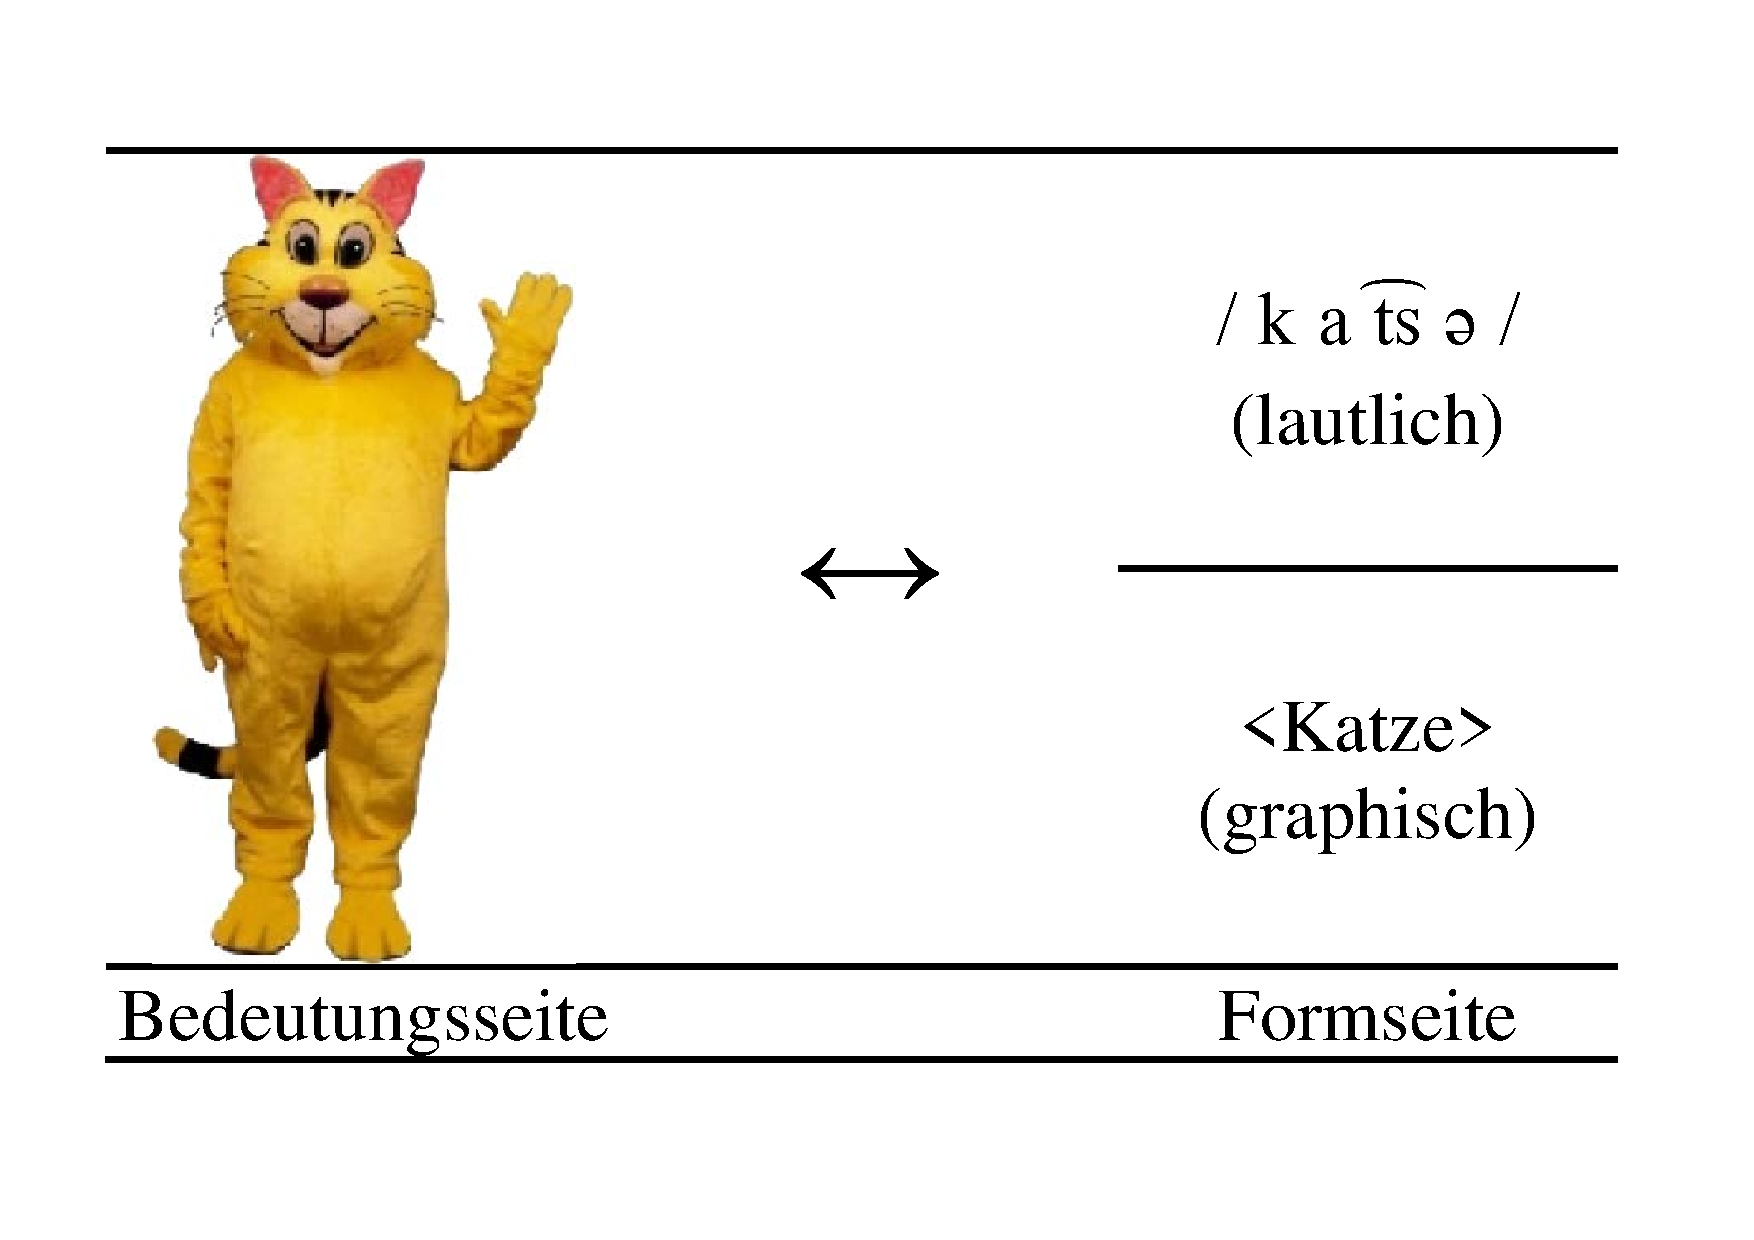
\includegraphics[scale=0.15]{material/01SSZeichenKatze}
%\caption{Beziehung zwischen Funktions-/Bedeutungs- und Formseite}
%\label{Zeichen1}
%\end{figure}

\end{frame}			


%%%%%%%%%%%%%%%%%%%%%%%%%%%%%%%%%%%
%Alternative zur Gelben Katze:

\begin{frame}
\frametitle{Sprachliche Zeichen: Form-Bedeutung-Paare}
\begin{table}
\huge
\centering
%\caption[Hauskatze]{https://commons.wikimedia.org/wiki/File:Hauskatze_an_einem_Scheunenfenster_in_Grossarl.JPG; Autor: Usien; GNU Free Documentation Licence}
\begin{tabular}{lp{1em}l}
\hline
\multirow{4}*{
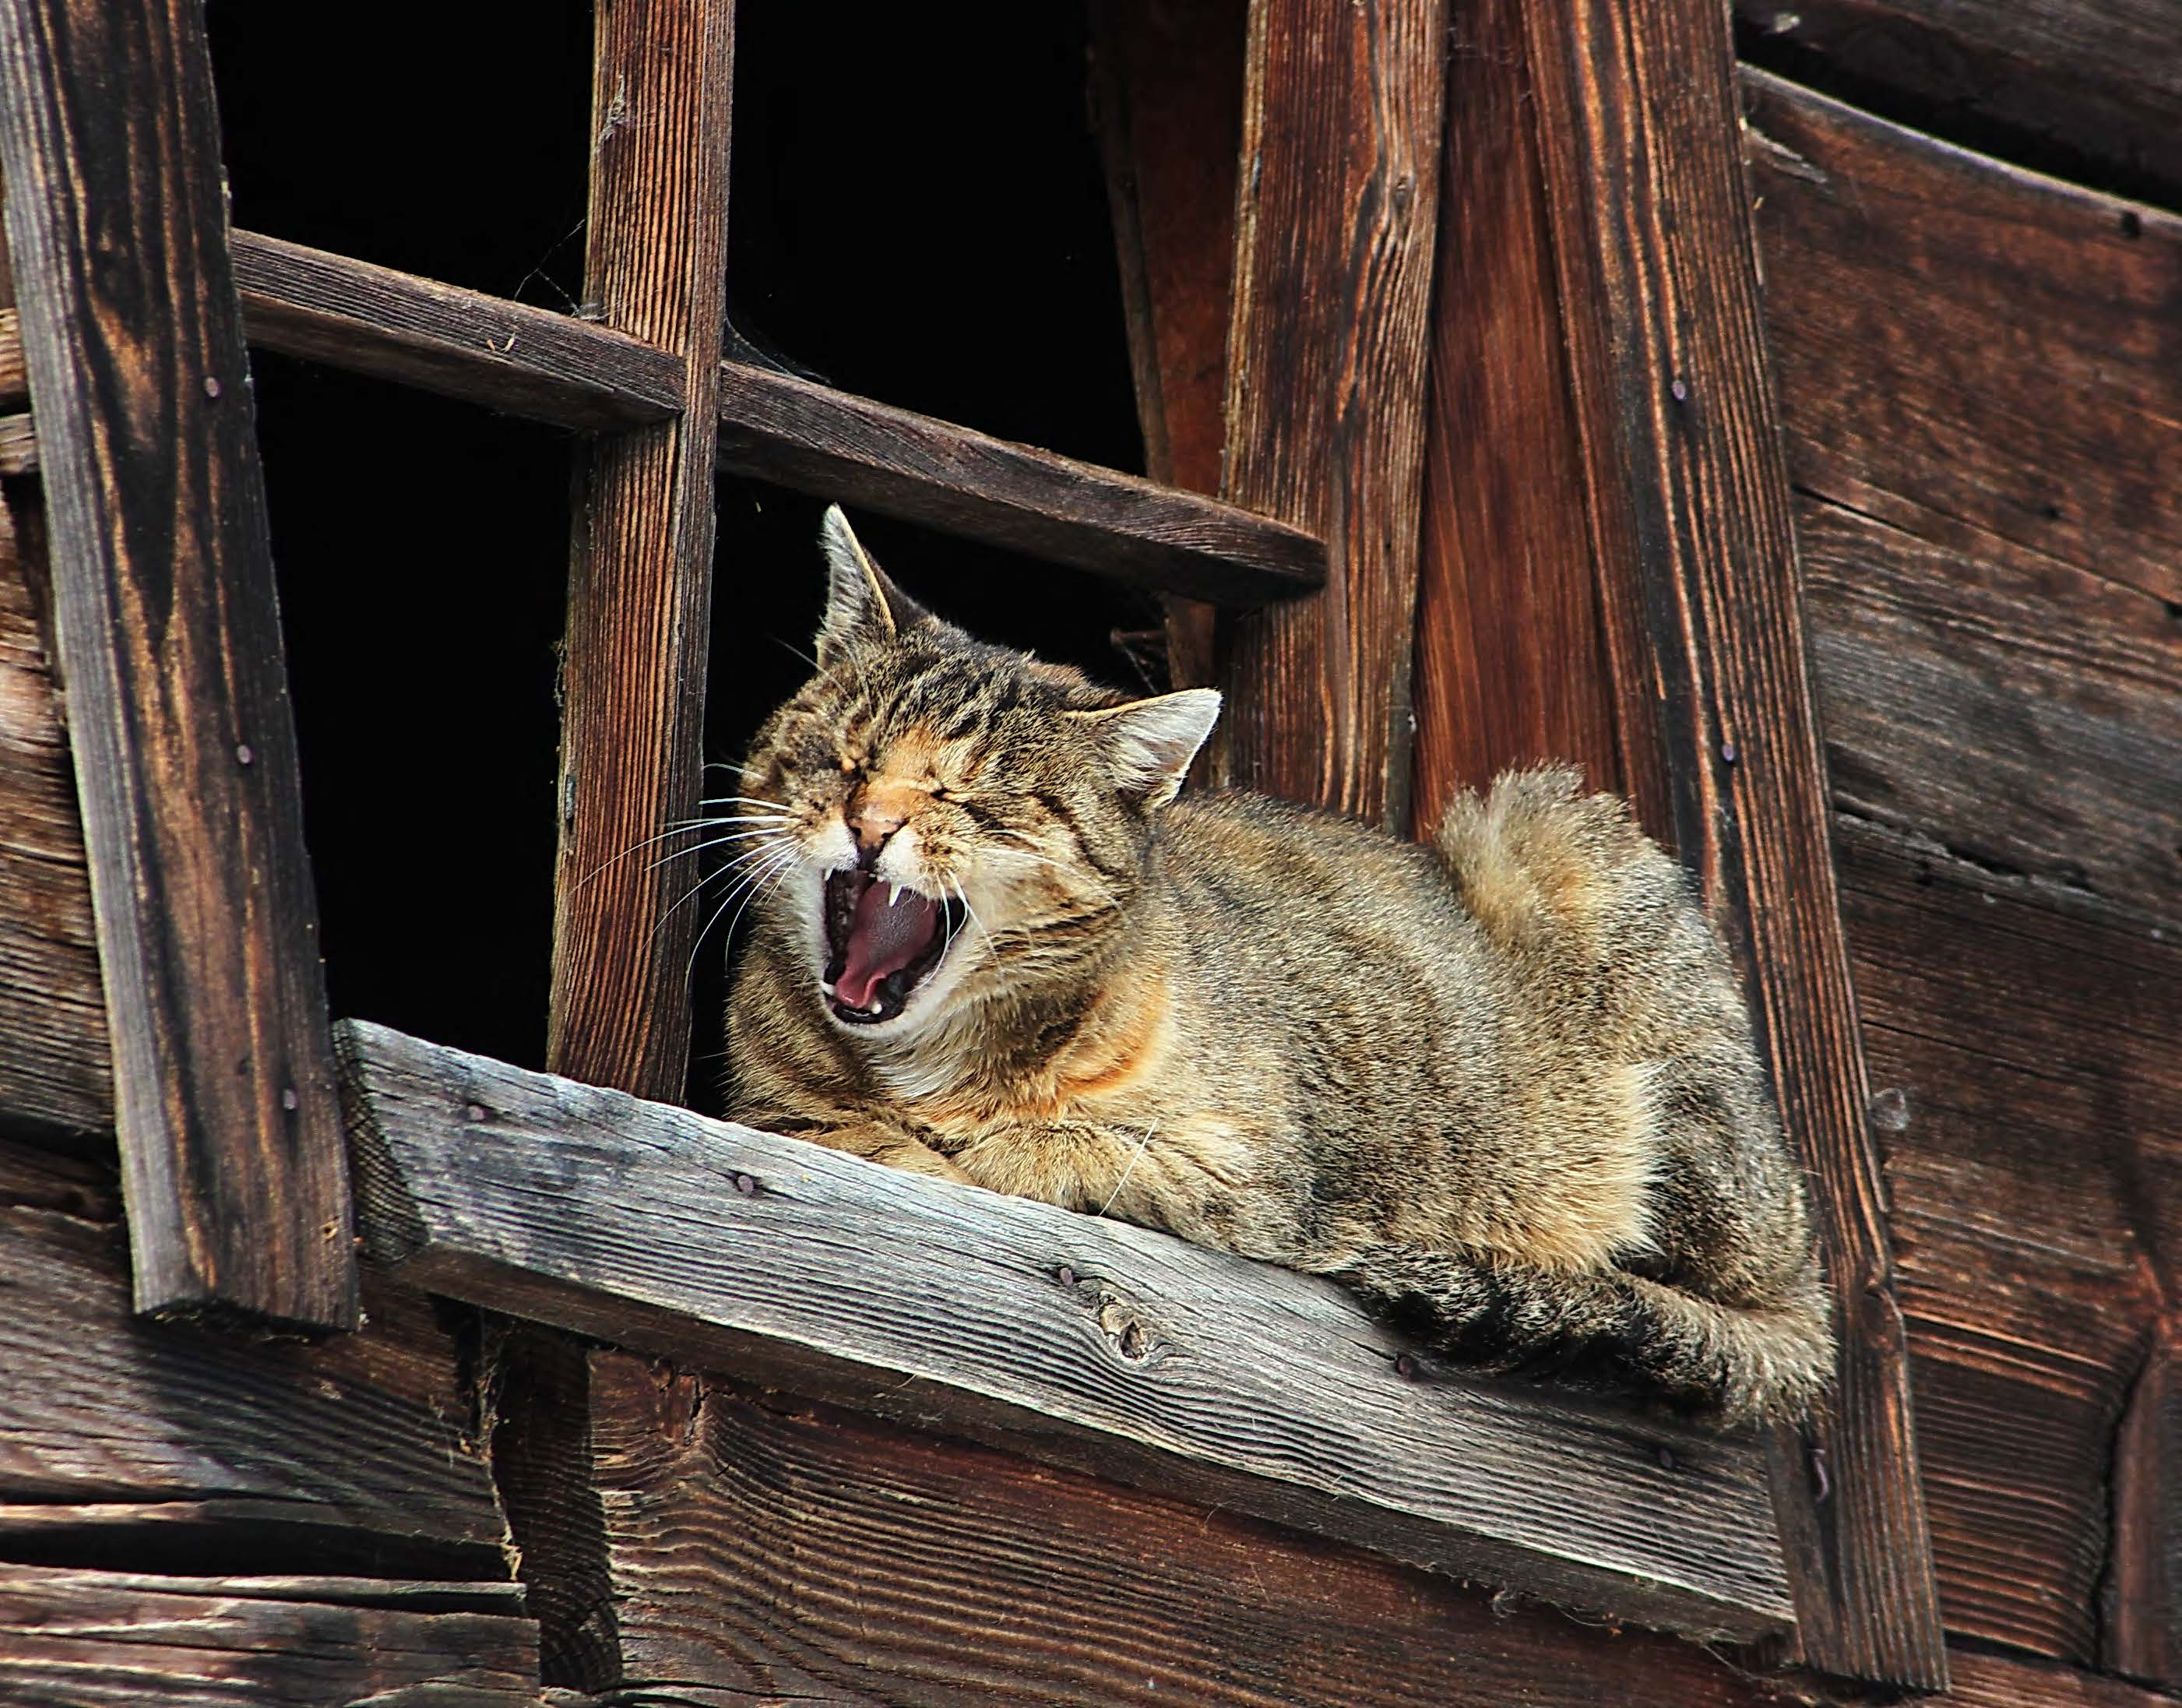
\includegraphics[scale=0.04]{material/Hauskatze-an-einem-Scheunenfenster-in-Grossarl}
}&  
%fehlt noch im Material-Ordner
\multirow{4}{6em}{{\Large $ \leftrightarrow $}} & / \textipa{k a \t{ts} \textschwa} / \\
                                              & &{\normalsize (lautlich)}\\
\cline{3-3}
& & $\langle$ Katze $\rangle$ \\
& & {\normalsize (graphisch)} \\
\hline
{\Large Bedeutungsseite} & & {\Large Formseite}\\
\hline \\
\end{tabular}
\end{table}

\hfill \dots vgl. \citet{Saussure16x}

\end{frame}


%%%%%%%%%%%%%%%%%%%%%%%%%%%%%%%%%%%
\begin{frame}
\frametitle{Zeichensysteme in der Tierkommunikation}

\begin{itemize}
	\item<1-> Tiere verwenden auch Zeichensysteme zur Kommunikation.
\end{itemize}			
			
%\begin{figure}[H]
%\centering

%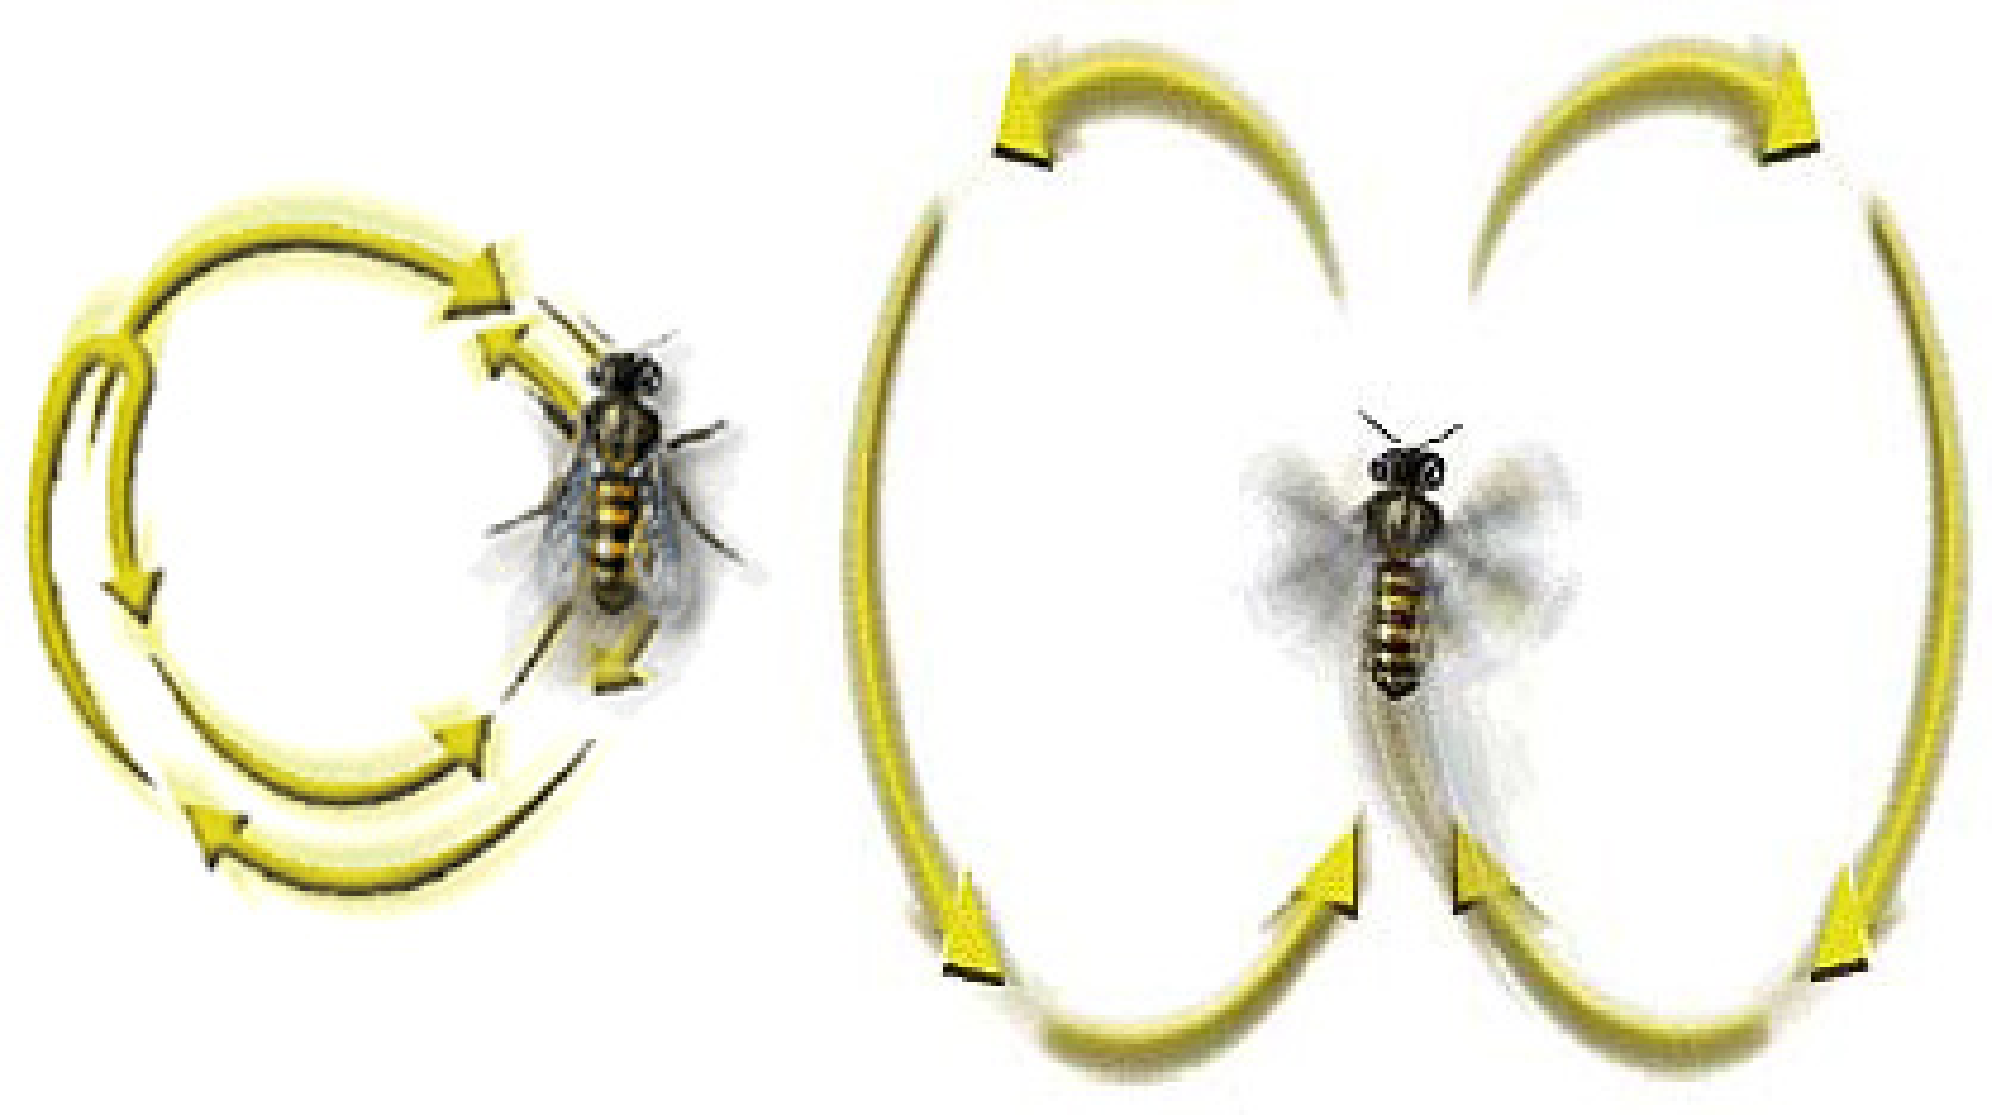
\includegraphics[scale=0.15]{material/01SSBienentanz}
%\caption{\gqq{Rundtanz} und \gqq{Schwänzeltanz} der Bienen}
%\label{Zeichen2}
%\end{figure}



\begin{itemize}
	\item<2-> Mit diesem Zeichensystem teilen Bienen die \textbf{Richtung} und \textbf{Entfernung} der nächsten Nahrungsquelle mit. 
	\item<2-> \textbf{Rundtanz:} Trachtgebiet in der Nähe (weniger als 25\,m)
	\item<2-> \textbf{Schwänzeltanz:} Trachtgebiet bis zu 10\,km weit entfernt, weitere Bewegungen zeigen die Richtung an.

\begin{figure}[H]
\centering
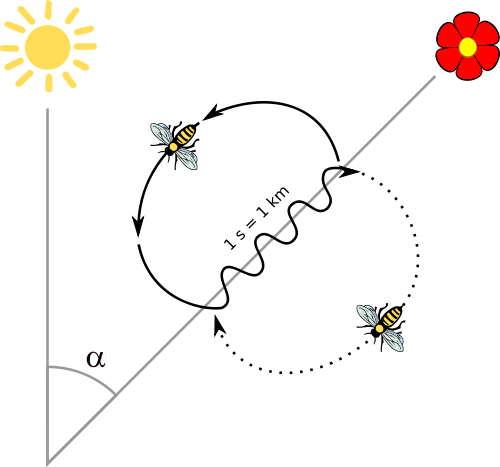
\includegraphics[scale=0.14]{material/Bee-dance}
%\caption{https://commons.wikimedia.org/wiki/File:Bee\_dance.png?uselang=de; GNU-Lizenz; Autor:Audriusa; Bee\_dance/Schwänzeltanz}
\label{Zeichen2}
\end{figure}

\end{itemize}		
		
\end{frame}			


%%%%%%%%%%%%%%%%%%%%%%%%%%%%%%%%%%%
\begin{frame}
\frametitle{Schwänzeltanz}

More than Honey. (R: Markus Imhoof, 2012), 13min 50sec.
%Quelle?

\end{frame}


%%%%%%%%%%%%%%%%%%%%%%%%%%%%%%%%%%%
%%%%%%%%%%%%%%%%%%%%%%%%%%%%%%%%%%%
\subsection{Merkmale natürlicher Sprachen}

%% MyP: Contents
\iftoggle{sectoc}{
	\frame{
		%\begin{multicols}{2}
		\frametitle{~}
		\tableofcontents[currentsubsection, subsubsectionstyle=hide]
		%\end{multicols}
	}
}

%% StM: Contents
\iftoggle{gliederung}{
	
	\outline{
		\begin{itemize}
			
			\item Ziel des Kurses
			\item Sprache und natürliche Sprache
			\item Zeichensysteme
			\item \blaubf{Merkmale natürlicher Sprachen}
			%% Bidirektionalität
			%% Situationelle Ungebundenheit
			%% Rückkopplung
			%% Diskretheit
			%% Produktivität
			%% Arbitrarität
			%% Fazit
			
		\end{itemize}
	}
}
%%%%%%%%%%%%%%%%%%%%%%%%%%%%%%%%%%%
	
\begin{frame}{Merkmale natürlicher Sprachen}

\begin{itemize}
	\item Die menschliche (natürliche) Sprache unterscheidet sich jedoch von anderen Zeichensystemen, wie der \gqq{Bienensprache} oder den Verkehrszeichen, \textbf{nicht in einem einzelnen Merkmal}, sondern \textbf{in einem Bündel von Merkmalen}, welche alle zusammen vorhanden sein müssen (vgl. \citealp{Hockett60a}).
\end{itemize}

\end{frame}


%%%%%%%%%%%%%%%%%%%%%%%%%%%%%%%%%%%
%%%%%%%%%%%%%%%%%%%%%%%%%%%%%%%%%%%
\subsubsection{Bidirektionalität}
%%% MyP: Contents
%\iftoggle{sectoc}{
%	\frame{
%		%\begin{multicols}{2}
%		\frametitle{~}
%		\tableofcontents[currentsubsubsection]
%		%\end{multicols}
%	}
%}
%%%%%%%%%%%%%%%%%%%%%%%%%%%%%%%%%%%

\begin{frame}{Bidirektionalität:}

	\begin{itemize}
		\item[]
		\item<1-> Mensch ist \textbf{sowohl Sender als auch Empfänger} eines Sprachsignals.
		\item[]
		\item<2-> Bei einigen Singvögeln ist das anders:
		
		\begin{itemize}
			\item[]
			\item[$\rightarrow$]<2-> Männchen singen zur Reviermarkierung oder um
                          Weibchen anzulocken.\\
                         Weibchen können oft nicht oder nur wenig singen.\\
                         Sie verstehen den Gesang der Männchen, können ihn aber selbst nicht produzieren.
		\end{itemize}
			
	\end{itemize}

\end{frame}


%%%%%%%%%%%%%%%%%%%%%%%%%%%%%%%%%%%
%%%%%%%%%%%%%%%%%%%%%%%%%%%%%%%%%%%
\subsubsection{Situationelle Ungebundenheit}
%%% MyP: Contents
%\iftoggle{sectoc}{
%	\frame{
%		%\begin{multicols}{2}
%		\frametitle{~}
%		\tableofcontents[currentsubsubsection]
%		%\end{multicols}
%	}
%}
%%%%%%%%%%%%%%%%%%%%%%%%%%%%%%%%%%%

\begin{frame}{Situationelle Ungebundenheit:}
	
	\begin{itemize}
		\item[]
		\item<1-> Menschen sind in der Lage auch über Dinge zu kommunizieren,\\
                          die \textbf{nicht hier und jetzt} stattfinden.
		
		\begin{itemize}
			\item[$\rightarrow$]<2-> Wir können über das leckere gestrige Essen in der Mensa und über unsere Freude auf das morgige Mensafestmahl reden.
		\end{itemize}
		\item<3-> Der Tanz der Bienen ist in diesem Fall der menschlichen Kommunikation ähnlich.
		\item<3-> Einige Primaten sind jedoch nur in der Lage über das Hier und Jetzt zu kommunizieren.
	\end{itemize}
		
\end{frame}


%%%%%%%%%%%%%%%%%%%%%%%%%%%%%%%%%%%
%%%%%%%%%%%%%%%%%%%%%%%%%%%%%%%%%%%
\subsubsection{Rückkopplung}
%%% MyP: Contents
%\iftoggle{sectoc}{
%	\frame{
%		%\begin{multicols}{2}
%		\frametitle{~}
%		\tableofcontents[currentsubsubsection]
%		%\end{multicols}
%	}
%}
%%%%%%%%%%%%%%%%%%%%%%%%%%%%%%%%%%%

\begin{frame}{Rückkopplung}
	
	\begin{itemize}
		\item<1-> Menschen können ihre \textbf{eigenen Sprachsignale} wahrnehmen und darauf reagieren.
		
\ea Ich habe heute \ldots ääähhhh GESTERN die Hausaufgaben abgegeben.
\z

\begin{itemize}
	\item<2->[$\rightarrow$] Der dreistachlige Stichling kann z.\,B. nicht die Färbung seiner Augen und seines Bauches wahrnehmen, die im Balzverhalten eine große Rolle spielt.
\end{itemize}
			\item[]
		\end{itemize}

\end{frame}


%%%%%%%%%%%%%%%%%%%%%%%%%%%%%%%%%%
%%%%%%%%%%%%%%%%%%%%%%%%%%%%%%%%%%
\subsubsection{Diskretheit}
%%% MyP: Contents
%\iftoggle{sectoc}{
%	\frame{
%		%\begin{multicols}{2}
%		\frametitle{~}
%		\tableofcontents[currentsubsubsection]
%		%\end{multicols}
%	}
%}
%%%%%%%%%%%%%%%%%%%%%%%%%%%%%%%%%%%

\begin{frame}{Diskretheit}
			
	\begin{itemize}
		\item Zeichen in natürlichen Sprachen können in kleine, diskrete (\textbf{voneinander unterscheidbare}) \textbf{Einheiten} zerlegt werden.

\pause
				
		\begin{itemize}
			\item[]
			\item[$\rightarrow$] \ab{Alben} und \ab{Alpen} unterscheiden sich nur in der Aussprache eines einzelnen Lautes.
			
			\ea \textipa{[\textglotstop{}al}{\red b}\textipa{@n]} vs. \textipa{[\textglotstop{}al}{\red p}\textipa{@n]}
			\z 
			
			\item[$\rightarrow$] Der Bienentanz ist eher kontinuierlich als diskret.						
		\end{itemize}
	
	\end{itemize}

\end{frame}


%%%%%%%%%%%%%%%%%%%%%%%%%%%%%%%%%%%
%%%%%%%%%%%%%%%%%%%%%%%%%%%%%%%%%%%
\subsubsection{Produktivität}
%%% MyP: Contents
%\iftoggle{sectoc}{
%	\frame{
%		%\begin{multicols}{2}
%		\frametitle{~}
%		\tableofcontents[currentsubsubsection]
%		%\end{multicols}
%	}
%}
%%%%%%%%%%%%%%%%%%%%%%%%%%%%%%%%%%%

\begin{frame}{Produktivität}
	
	\begin{itemize}
		\item<1-> Eins der wichtigsten Merkmale natürlicher Sprachen!
%		\item[]
		\item<2-> Aus einer \textbf{begrenzten Menge} von \textbf{Lauten} wird eine von
                  Menschen nicht überschaubare Menge von \textbf{Wörtern} und daraus eine unüberschaubare Menge von \textbf{Sätzen} produziert ($\rightarrow$ offenes oder produktives System).
%		\item[]
		\item<2-> Menschen können noch nie gehörte Sätze verstehen und noch nie gesagte Sätze produzieren.

\pause

\ea Meine Freundin hat gestern einen Wasserkocher mit Treueherzen von Kaiser's gekauft.
\ex Meine Freundin von Kaiser's hat gestern Treueherzen mit einem Wasserkocher gekauft.
\z
				
	\item<3-> Der Gibbon (kleiner Menschenaffe) hat ein geschlossenes Rufsystem mit einem kleinen \textbf{endlichen Inventar} an bekannten Lauten. 
	
	\end{itemize}
\end{frame}


%%%%%%%%%%%%%%%%%%%%%%%%%%%%%%%%%%%
%%%%%%%%%%%%%%%%%%%%%%%%%%%%%%%%%%%
\subsubsection{Arbitrarität}
%%% MyP: Contents
%\iftoggle{sectoc}{
%	\frame{
%		%\begin{multicols}{2}
%		\frametitle{~}
%		\tableofcontents[currentsubsubsection]
%		%\end{multicols}
%	}
%}
%%%%%%%%%%%%%%%%%%%%%%%%%%%%%%%%%%%

\begin{frame}{Arbitrarität}

\begin{itemize}
	\item<1-> \textbf{Bezeichnendes} (Signifikant, frz.\ signifiant) ist nicht durch \textbf{Bezeichnetes} (Signifikat, frz. signifié) bestimmt.
	\item[]
	\item<2-> Verschiedene Sprachen haben unterschiedliche Namen (Bezeichnendes) für das gleiche Objekt (Bezeichnetes):

\pause

\ea dt. \ab{Stift}, engl. \ab{pen}, sp. \ab{bolígrafo}, frz. \ab{crayon}, \ldots
\z

\pause 

	\item Benennung ist \textbf{konventionell}, \dash in der Sprachgemeinschaft festgelegt.

	\begin{itemize}
		\item[$\rightarrow$] Der Tanz der Bienen ist nicht arbiträr, sondern motiviert.
	\end{itemize}

\pause
		
	\item Es gibt in natürlichen Sprachen \textbf{auch motivierte} Zeichen:

\ea Deutsch und Dänisch \textipa{[va\textupsilon{} va\textupsilon{}]}, Griechisch \textipa{[gav gav]}, Russisch \textipa{[gaf gaf]}, Spanisch \textipa{[g\textupsilon{}au g\textupsilon{}au]}, Französisch \textipa{[g\textupsilon{}af g\textupsilon{}af]}, Englisch \textipa{[w\textopeno{}f w\textopeno{}f]}, Litauisch \textipa{[a\textupsilon{} a\textupsilon{}]}, Koreanisch \textipa{[m\textopeno{}N m\textopeno{}N]}
\z

\end{itemize}

\end{frame}


%%%%%%%%%%%%%%%%%%%%%%%%%%%%%%%%%%%
%%%%%%%%%%%%%%%%%%%%%%%%%%%%%%%%%%%
\subsubsection{Fazit}
%%% MyP: Contents
%\iftoggle{sectoc}{
%	\frame{
%		%\begin{multicols}{2}
%		\frametitle{~}
%		\tableofcontents[currentsubsubsection]
%		%\end{multicols}
%	}
%}
%%%%%%%%%%%%%%%%%%%%%%%%%%%%%%%%%%%
\begin{frame}{Fazit}
		
	\begin{block}{Natürliche Sprache}
			Insgesamt bildet die natürliche Sprache also ein \textbf{produktives}, \textbf{bidirektionales}, \textbf{arbiträres} und \textbf{diskretes} Symbolsystem (vgl. \citealp{Luedeling2009a}).
	\end{block}

\end{frame}	

%%%%%%%%%%%%%%%%%%%%%%%%%%%%%%%%%%%
%\begin{frame}{Übung}
%	Wie unterscheiden sich Computersprachen von natürlichen Sprachen? Diskutieren Sie dies anhand der eingeführten Kriterien.
%\end{frame}
%
%%%%%%%%%%%%%%%%%%%%%%%%%%%%%%%%%%%
%\iftoggle{ue-loesung}{
%	
%\begin{frame}{Übung -- Lösung}
%Wie unterscheiden sich Computersprachen von natürlichen Sprachen? Diskutieren Sie dies anhand der eingeführten Kriterien.
%
%{\red
%	
%\begin{itemize}
%\item Produktivität: ja, 
%\item Bidirektionalität:
%\item Arbitrarität: 
%\item Diskretheit: 
%\end{itemize}
%
%}
%
%\end{frame}
%
%}

%%%%%%%%%%%%%%%%%%%%%%%%%%%%%%%%%%%
%%%%%%%%%%%%%%%%%%%%%%%%%%%%%%%%%%%
\subsection*{Quellen}
%%%%%%%%%%%%%%%%%%%%%%%%%%%%%%%%%%%

\begin{frame}{Quellen}
	
	
	\begin{itemize}
		\item ABBILDUNG -- \gqq{Hauskatze} (Zugriff: 02.08.2019): \url{https://commons.wikimedia.org/wiki/File:Hauskatze\_an\_einem\_Scheunenfenster\_in\_Grossarl.JPG}
		%\medskip
		\item ABBILDUNG -- \gqq{Bienentanz} (Zugriff: 02.08.2019):
		\url{https://commons.wikimedia.org/wiki/File:Bee\_dance.png?uselang=de}
                \item VIDEO -- 	\textit{More than Honey}. Regie: Markus Imhoof. Drehbuch: Markus Imhoof, Kerstin Hoppenhaus. Schweiz/Deutschland/Österreich 2012. Fassung: DVD, 95 Min.
	\end{itemize}	
	
\end{frame}


%% %%%%%%%%%%%%%%%%%%%%%%%%%%%%%%%%%%%
%% %%%%%%%%%%%%%%%%%%%%%%%%%%%%%%%%%%%
%% \subsection*{Elektronische Quellen}
%% %%%%%%%%%%%%%%%%%%%%%%%%%%%%%%%%%%%

%% \begin{frame}{Elektronische Quellen}
	
	
	
%% 	\begin{itemize}
%% 		\item VIDEO -- 	\textit{More than Honey}. Regie: Markus Imhoof. Drehbuch: Markus Imhoof, Kerstin Hoppenhaus. Schweiz/Deutschland/Österreich 2012. Fassung: DVD, 95 Min.
%% 	\end{itemize}
	
%% \end{frame}

